
\documentclass[UTF8]{article}
\usepackage{xeCJK}
\usepackage{amsmath,amssymb}
\begin{document}

   \section{语法感知即时代码完成}       \label{sec:approach}   

在本节中,我们将概述我们的语法感知即时 Python 代码完成方法 (   \our   )。

从概念上讲,   \our    ~旨在不管源代码的完整性如何随时生成源代码,同时在学习阶段考虑源代码的句法和语义信息,但在推理阶段不需要句法信息。为了确保学习过程同时考虑语义和句法信息,我们将方法设计为专注于两个预测任务,即代码标记预测任务和标记类型预测任务。特别是,我们利用多任务训练技术 (MTT) 来协同学习代码标记预测任务(任务 1:预测下一个代码标记,视为目标任务)和标记类型预测任务(任务 2:预测它的令牌类型,被视为支持任务)。对于类型预测任务,我们建议利用标准的 Python 令牌类型信息(例如,字符串、数字、名称、关键字),这些信息很容易获得且轻量级,而不是使用我们发现不可用于三分之二的执行(请参阅我们在    \ref{sec:motivation}    节中的发现),限制了其执行即时代码完成的能力。相比之下,我们的    \our    ~ 在推理阶段不需要句法信息。因此,不需要推理时源代码的完整性。

概述。图~    \ref{fig:overview}    展示了我们的    \our    的概览,它包括两个阶段:训练和推理。在训练阶段,   \our    ~执行 6 个主要步骤: 步骤~    \circled{1}    类型提取,从源代码中提取令牌类型信息; Step~    \circled{2}    Tokenization,对源码进行subword tokenization; Step~    \circled{3}    Data Alignment,将字级别的类型信息与当前子字级别的代码信息对齐; Step~    \circled{4}    Multi-task Training Architecture with 3 training techniques: hard parameters sharing (MTL), soft parameters sharing (MTL), and intermediate fine-tuning (IFN); 然后在Step~    \circled{5}    Hyperparameter Task Weighting and Step~    \circled{6}    Decoding Methods是最大化性能的探索步骤。对于推理阶段,我们在Step~   \circled{7}    Code Generation步骤中描述了token-level预测和line-level预测的细节。

   \begin{figure*}
    \centering
    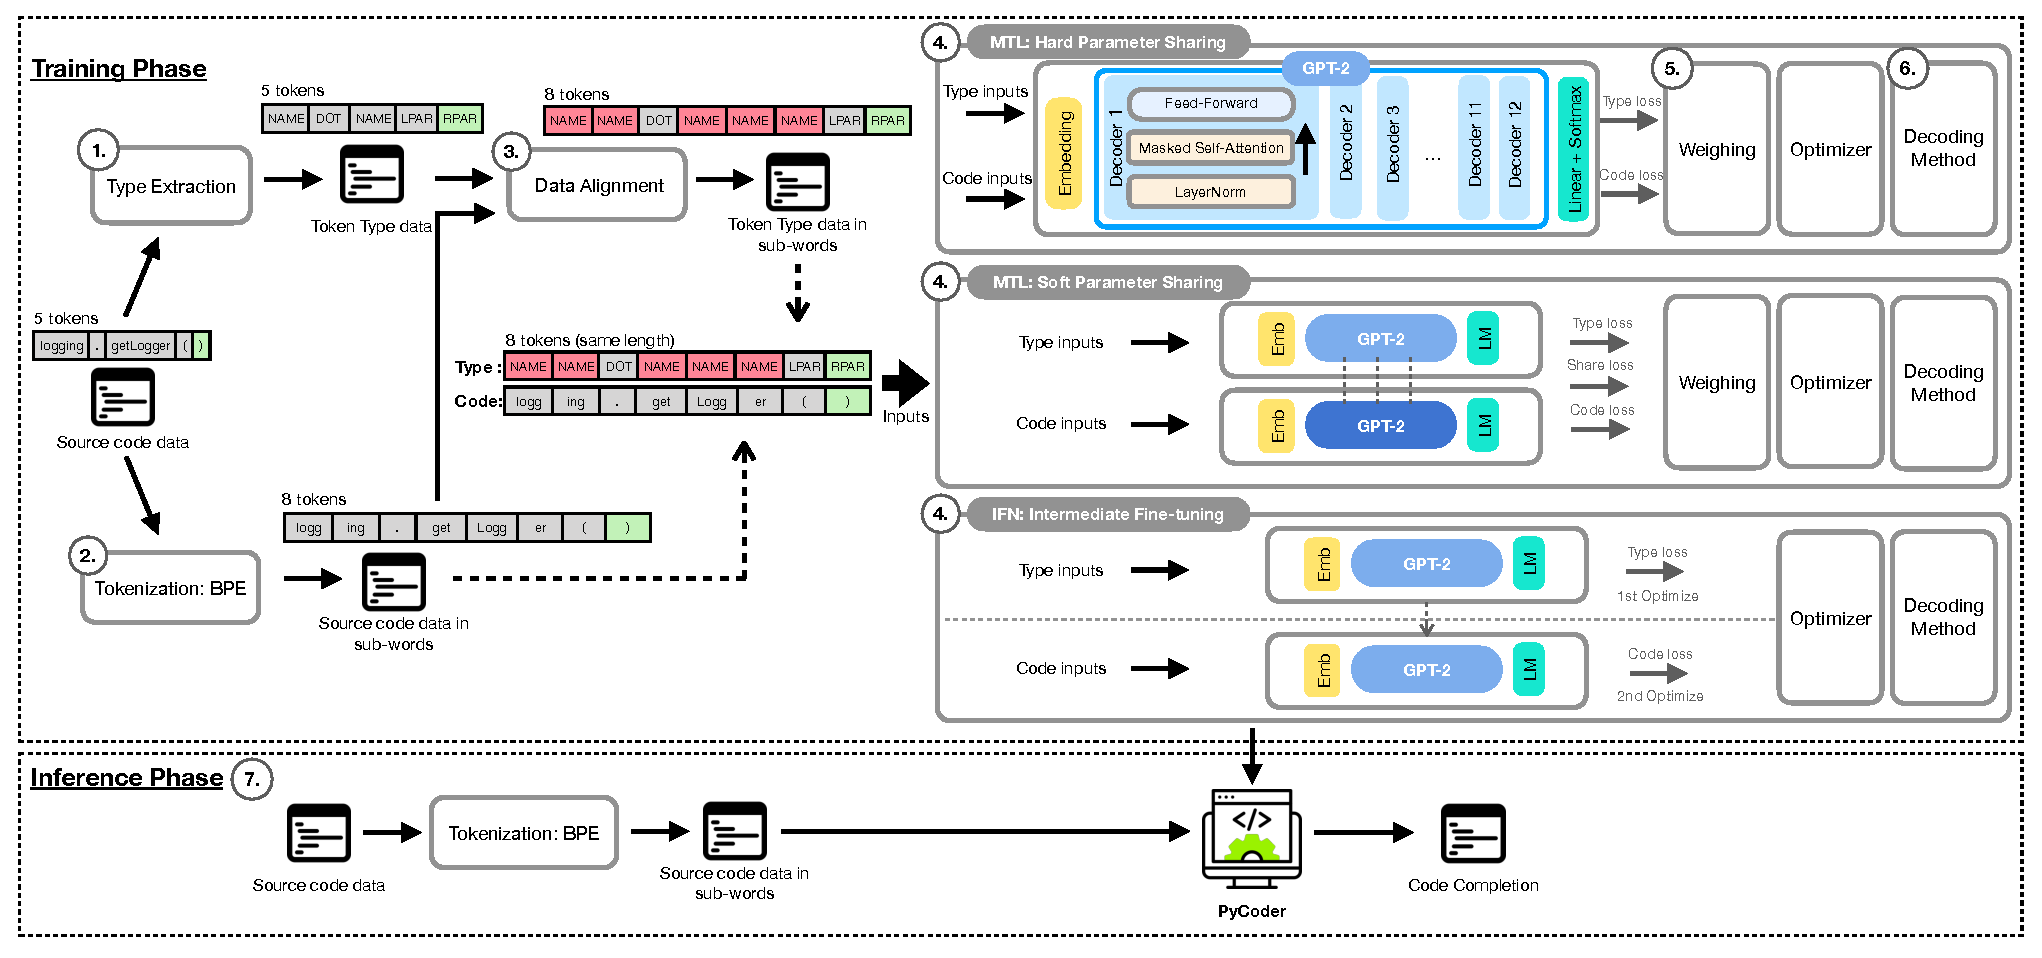
\includegraphics[width=\textwidth]{figures/overview.pdf}
    \caption{我们的语法感知即时 Python 代码完成方法 (PyCoder) 的概述。}
    \label{fig:overview}
\end{figure*}   

   \subsection{(步骤 1)类型提取}   

句法信息可以用多种形式表示,例如,在以前的工作中广泛使用的抽象语法树(AST),以及很大程度上未被探索的令牌类型信息。事实上,AST 和 token 类型信息都各有优缺点。虽然 AST 提供了源代码语法信息的形式化表示,但它需要语法正确的源代码才能被 Python AST 解析器成功解析。由于我们在    \ref{sec:motivation}    节中的发现表明 Python AST 解析器无法对开发人员键入的三个字符中的每两个字符执行一次,因此现有的基于 AST 的代码完成方法的使用场景在实践中仍然受到限制。

为了应对这一挑战,我们利用标准的 Python 令牌类型信息,提供源代码语法结构的更抽象表示(例如,名称、字符串、数字),其中 (1) 更轻量级,(2) 遵循自然代码序列的顺序; (3) 可以在任何时候被成功解析,而不需要完整和语法正确的源代码。通常,标准 Python 令牌由两部分信息组成,即 (1) 提供句法含义的令牌类型,以及 (2) 提供语义含义的令牌值。例如,给定一个    \texttt{logging}    令牌,令牌类型是    \texttt{NAME}    并且它的值是    \texttt{logging}    。由于令牌类型信息在现有代码完成基准中不可用,我们在下面描述提取类型信息的步骤。

为了提取类型信息,我们使用标准 Python 标记器库    \footnote{https://docs.python.org/3/library/tokenize.html}    提供的    \texttt{tokenizer}    函数和一个选项    \texttt{exact\_type}    以便为每个标记提取最细粒度的类型。对于 Python 分词器(Python 3.7 版本),总共将有 58 种不同的类型。特别地,我们关注以下 12 种主要类型的代码标记:   \texttt{<NAME>}   、   \texttt{<NUMBER>}   、   \texttt{<STRING>}   、   \texttt{<INDENT>}   、   \texttt{<DEDENT>}   、   \texttt{<ERRORTOKEN>}   、   \texttt{<ENDCODING>}   、   \texttt{<ENDMARKER>}   、   \texttt{<COMMENT>}   、   \texttt{<NL>}   、   \texttt{<NEWLINE>}    和    \texttt{<OP>}   X操作类型(例如,operator.delimiter),例如    \texttt{<LESS>}    、    \texttt{<GREATER>}    、    \texttt{<EQUAL>}    、    \texttt{<DOT>}    。然后,我们执行以下预处理步骤。

   \begin{itemize}   \item    首先,我们丢弃以下三种不会被执行的token类型,即描述Python文件编码的   \texttt{<ENCODING>}   、描述Python文件结束位置的   \texttt{<ENDMARKER>}   和描述Python文件代码注释的   \texttt{<COMMENT>}    .
    \item    其次,Python 分词器提供的    \texttt{<NAME>}    可以是标识符名称(例如    \texttt{logging}    )或 Python 保留名称(例如    \texttt{True}    )。因此,代码完成方法可能无法识别标识符名称和 Python 保留名称之间的区别——这并不反映现实。为了确保我们的代码完成方法能够识别不同类型名称之间的差异,我们使用    \texttt{keyword.iskeyword()}    函数    \footnote{https://docs.python.org/3/library/keyword.html}    来检查并将最初提取为    \texttt{<NAME>}    的所有 Python 保留字重命名为    \texttt{<KEYWORDS>}    。
    \item    第三,由于 CodeXGLUE~    \cite{lu2021codexglue}    基准数据集对任何新行一视同仁,我们还将    \texttt{<NEWLINE>}   (新行)、   \texttt{<NL>}   (新空白/注释行)转换为    \texttt{<EOL>}   (行尾)。\end{itemize}   

使用这种方法,令牌类型的表示(即每个令牌都有自己的类型)遵循源代码的自然顺序,而不是 AST 结构,它解决了基于 AST 的代码完成方法的局限性。如图~    \ref{fig:overview}    所示,   \texttt{logging.getLogger()}    将被标记为    \texttt{[logging, ., getLogger, (, )]}   ,具有以下标记类型    \texttt{[NAME, DOT, NAME, LPAR, RPAR]}   。

   \subsection{(步骤 2)令牌化}    Tokenization 是自动代码完成的重要步骤,旨在将源代码拆分为有意义的单元。粒度一般分为三个级别,即词级别、子词级别和字符级别。虽然词级表示是最简单的标记化方法,但它可能会产生大量的词汇量。但是,根据频率限制词汇量可能会导致词汇外词 (OOV) 问题。虽然字符级表示可以减少词汇量有限(例如英文字符)的 OOV 问题,但模型可能无法处理过长的源代码序列(即每个字符都有自己的向量)。相反,我们使用字节对编码 (BPE) 算法的子词标记化~    \cite{sennrich2015neural}   ,因为先前的研究发现 BPE 可以大大减少词汇量~    \cite{fu2022gpt2sp, karampatsis2020big}   ,同时能够生成从未出现在数据集中的新标识符~    \cite{thongtanunam2022autotransform}   。首先,BPE 将源代码拆分为字符。然后,BPE 根据出现的频率迭代地将字符合并到子词中,以创建词汇表,直到达到所需的大小。在本文中,我们使用 CodeGPT 分词器,它的词汇量为 50,000 个子词。为确保 CodeGPT 分词器可以识别标记类型,我们在方括号    $\langle...\rangle$    中表示标记类型,它们包含在 BPE 分词器的特殊标记词汇表中,以避免对这些标记类型进行任何子词分词。

   \subsection{(步骤 3)数据对齐}    数据对齐是确保代码令牌的序列及其对应的令牌类型正确匹配和对齐的重要步骤。使用BPE,一些词可能被标记为子词,而它们的类型没有被标记到子词级别,导致代码标记序列和相应的标记类型无法正确匹配。例如,如图~    \ref{fig:overview}    所示,BPE 将    \texttt{logging}    拆分为    \texttt{[logg, ing]}   ,并具有单个对应的    \texttt{<NAME>}    标记类型。为了解决这个问题,我们对任何被 BPE 拆分的单词重复标记类型。因此,在图~    \ref{fig:overview}    中,token 类型    \texttt{<NAME>}    重复了两次,以匹配    \texttt{[logg, ing]}    的子字级代码序列。此数据对齐步骤将生成一系列代码标记及其相应的具有相同长度的标记类型,这些标记已准备好输入我们的代码完成方法以学习源代码的句法和语义含义。

   %! Author = sbbfti
%! Date = 10/06/2020

% \subsection{Models}
% \textit{finish} \kla{reviewers could argue that some other models learn both syntactic and semantic information. If this model only learns syntactic, how are they going to be accurate? check existing work why they call they learn semantic information and see if ours also learn semantic information or not. Otherwise, we are downtown the claim.}

% \kla{should we talk about two prediction tasks somewhere? Task1=? and Task2=}

\subsection{(Step 4) Multi-Task Training Architectures}
\label{sec:approach-arch}


% On the other hand, training multiple single models on multiple tasks is also possible, but predictions are competing and the multiple sources of information are not jointly learned together, leading to inaccurate predictions.



Our \our~leverages a Multi-Task Training (MTT) paradigm, which is a set of techniques designed to learn multiple tasks, allowing the model to capture multiple sources of information.
Traditionally, deep learning is designed for one single learning objective (e.g., only predicting the next code token), limiting its ability to capture other important and useful sources of information (e.g., syntactic information of source code).
Instead of training a model with one single learning objective, the MTT paradigm aims to provide a generalist model with multiple learning objectives, providing a more robust vector representation.
For our \our~approach, we design the target task to predict the next token, while the supporting task (aka. an auxiliary task or additional related non-target task) is to predict the token type.
In addition, we build three variants of \our, with three different MTT techniques, according to two learning styles~\cite{phang2018sentence} as follows.
% (i.e., \our-Hard, \our-Soft, and \our-IFN)

\subsubsection{Multi-Task Learning (MTL)}

Multi-Task Learning (MTL) is an MTT technique to learn multiple tasks simultaneously instead of learning them separately.
Normally, during the learning process, the model aims to optimize a loss function for one single learning objective.
With the MTL approaches, multiple loss functions are optimized together during the learning process, allowing the MTL-based model to simultaneously learn against multiple objectives and share the knowledge understanding from multiple related sources.
In this paper, we consider two main MTL approaches for Multi-Task Learning (MTL)~\cite{ruder2017overview}, i.e., Hard Parameter Sharing (\our-Hard) and Soft Parameter Sharing (\our-Soft).

For \emph{Hard Parameter Sharing}, the key principle is to train a code completion model against two learning objectives, where the loss functions of the two learning objectives ($L_{code}$ and $L_{type}$) are optimized together within the same model.
Formally, the \our-Hard model aims to minimize the following loss function: 
\begin{equation}
    \label{eq:1} 
    \begin{aligned}
    \medmath{L_{Hard} = \argmin_{\omega}(L_{code}(d_{code}, \omega) + L_{type}(d_{type}, \omega))}
    % loss_{hardShare} = codeLoss + typeLoss
    \end{aligned}
\end{equation} 

\noindent , where $d_{code}, d_{type}$ denotes the code token dataset and the token type dataset, respectively, and $\omega$ denotes a model's parameters.
With Hard Parameter Sharing, the weights and model parameters are shared between tasks, allowing the model to explicitly learn the input representations between tasks (i.e., code and type vectors) that are closely related.



% via the shared layers which may help enhance the effectiveness of the target task's results.
% After the shared layers, usually there are separated task-specific output layers for each task.
% However for our work, the tasks have similar outputs i.e. tokens from the vocabulary.
% Therefore, we train both target task and supporting task in the same model simultaneously without separated output layer.

% SynComp hard parameter sharing uses one GPT-2 model with two losses: code prediction loss ($L_{code}$) and type prediction loss ($L_{type}$).
% The model minimize the summation of losses shown in Equation~\ref{eq:1}.



% For hard parameter sharing, the tasks will share the same model backbone which mean the weights and parameter of the model being shared together.
% Only the task-specific output layer that might be different.
% A hard parameter sharing model is one of the most popular multi-task learning techniques.
 

% \kla{wannita will write soft....}

% \subsubsection{MTL: Soft Parameter Sharing Model}
% For soft parameter sharing, each task will have its own model backbone, i.e. separate weights and parameters.
% However, the models are loosely connected by the constraint which try to minimize the distance of the model parameters' difference.
% This is to regularize the model parameters to be similar.
For \emph{Soft Parameter Sharing}, the key principle is similar to Hard Parameter Sharing where the goal is to train a code completion model with two learning objectives.
However, instead of training a model against two tasks like the Hard Parameter Sharing model, the Soft Parameter Sharing is designed to train two individual models for each task ($L_{code}$ and $L_{type}$), allowing each model to learn separately for each task.
Therefore, each learning objective has an individual model (i.e. separated weights and parameters between the learning objectives).
% to learn and predict outputs; 
To allow the model to share the knowledge between tasks (i.e., to learn the similarities between the related parameters), a shared loss function is also used, which is computed as follows:

\begin{equation}
    \label{eq:norm}
    L_{sharing}(\omega_1, \omega_2) = 
    % ||W||_F = 
    \sqrt{\sum_{i=1}^{I}\sum_{j=1}^{J}|\omega_{1(i,j)}-\omega_{2(i,j)}|^2}
\end{equation}

% Nonetheless, the models are loosely connected by the constraint to encourage similarities between related parameters.


% The constraint ($L_{sharing}$) which is used to optimize the difference of distance between the models parameters' applies with Frobenius norm:

\noindent , where $\omega_n$ denotes the model parameters of the  learning objective $n$. Finally, the \our-Soft model aims to minimize the following loss function:

\begin{equation}
\label{eq:2}
\begin{aligned}
    L_{Soft} = \argmin_{\omega_1, \omega_2}
    &( L_{sharing}(\omega_1, \omega_2)\\ 
    &+ L_{code}(d_{code}, \omega_2)\\
    &+ L_{type}(d_{type}, \omega_1))
\end{aligned}
\end{equation}

With Soft Parameter Sharing, each learning objective has its own model parameters and weights, allowing the models to implicitly learn the input representations that might have more connection to a specific task.

% SynComp soft parameter sharing uses two GPT-2 models with three losses: code prediction loss, type prediction loss, and sharing loss. The model minimize the summation of losses shown in Equation~\ref{eq:2}.

\subsubsection{Intermediate Fine-Tuning (IFT)}

\emph{Intermediate Fine-Tuning (IFT)}~\cite{phang2018sentence} adapts a transfer learning concept (i.e., pre-training then fine-tuning) where the goal is to learn multiple tasks sequentially. First, the model is fine-tuned on the supporting task (token type prediction) followed by the target task (code token prediction), respectively.
Thus, the fine-tuned step on the supporting task can be considered the second stage of the model pre-training.
Therefore, the Intermediate Fine-Tuning (IFT) model (\our-IFT) is first trained based on an intermediate self-supervised task (token type prediction), then trained on the target task (code token prediction), allowing the model to gain knowledge on the token type prior to predicting the next code tokens.


\subsection*{GPT-2 Model Architecture}

Among the three variants of the MTT techniques (i.e., \our-Hard, \our-Soft, and \our-IFT), we use the GPT-2 architecture as a base model.
GPT-2~\cite{radford2019language} is a decoder-only Transformer model.
The GPT-2 architecture for code completion consists of three main components: the embedding layer, the decoder block, and the language model head. 
First, the embedding layer embeds the input tokens into vectors with positional encoding, allowing the model to learn the semantic meaning and the position of each code token.
Then, the embedding vectors are fed into the decoder block which contains decoder layers.
Each decoder layer includes masked self-attention layers, feed-forward neural network layers, and normalization layers.
%  It basically always scores the future tokens as 0 so the model can’t peak to future words
The masked self-attention layer indicates which tokens to focus on, while the masking approach prevents the attention mechanism~\cite{vaswani2017attention} to see the unseen tokens in the future.
% \kla{wannita will do the rest}.
% Feedforward neural nets are complex network made up an input layer that accepts information, hidden layers that capture the hidden correlations between each data point, and an output layer which transmit information.
The feed-forward neural network layer is a sophisticated network with hidden nodes to capture the related information between each data point.
% Layer normalization (LayerNorm) is a technique to normalize the distributions of intermediate layers. It enables smoother gradients, faster training, and better generalization accuracy.
The normalization layer makes the learning process more effective by enabling smoother gradients and generalized accuracy.
% The linear layer takes the output of the last decoder block and converts it to a vector whose dimensions are vocabulary size by 1. In short, it takes a lot of inputs and produces a list where each spot represents a token. The higher the number in the spot the better the chance that that token is the best pick. Softmax converts the output of the linear layer to a probability distribution
After $L$ layers of decoder, an output of the last layer is fed to the language model head, i.e. a linear layer, which converts the output to a vector whose dimensions are the same as the vocabulary size.
Lastly, the vector is converted to a probability distribution by the softmax activation function.
Formally, to predict the next token $x_t$ based on a given input sequence, GPT-2 can be represented as follows:

\begin{equation}
\begin{aligned}
    \label{eq:transformer}
    h_0 &= W_e \cdot C + W_p \\
    % \label{eq:transformer2}
    h_l &= decoder\_layer(h_{l-1}), \forall l \in [1,L] \\
    % \label{eq:transformer3}
    P(x_t) &= y_t = softmax(h_n \cdot W^T_e), t \in [0, N]
\end{aligned}
\end{equation}

\noindent, where $W_e$ is the tokens embedding matrix, $C$ denotes the context vector of tokens, $W_p$ is the position embedding matrix, $L$ is a number of decoder layers, and $N$ is the length of the sequence.
We follow the traditional language models by maximizing the log-likelihood of:

\begin{equation}
    \label{eq:log-likelihood}
    L(x_t) = \sum_i{\log P(x_i|x_1...x_{i-1}, \omega)}
\end{equation}

\noindent, where $\omega$ is the model parameters that are learned during the optimization process.
Particularly, \our~uses the pre-train CodeGPT~\cite{lu2021codexglue} that is pre-trained on the CodeSearchNet dataset~\cite{husain2019codesearchnet} as a starting checkpoint.


% Below we provide details for each training techniques.



% In Fig.~\ref{fig:overview} shows the architectures of all described models.
% During the training phase, both tasks are cooperatively trained; however, the task can separately predict in the inference phase as shown in Fig.~\ref{fig:overview}.
% In other words, the token type information is used only to support throughout the training phase requiring no token type extraction in the inference phase.
% which yield to the benefit of on-the-fly model by not requiring token type extraction in the inference phase.

% SynComp has GPT-2~\cite{radford2019language}, a Transformer decoder-only model, as a based model for all techniques.
% The based model consist of three main components: embedding layer, decoder block, and language model head. 
% Before handing that to the first block in the model, we need to incorporate positional encoding – a signal that indicates the order of the words in the sequence to the transformer blocks.



% \gls{ifn} is adapted from transfer learning paradigm which is about pre-training and then fine-tuning on target task.
% Specifically, this is the training technique for sequential training.
% The model is fine-tuned on supporting tasks and then target task respectively.
% This technique benefit the model to learn the second stage of pre-training with intermediate supervised task that might mitigate the brittleness and improve the robustness and performance of the target task~\cite{phang2018sentence}.

% In our case, SynComp intermediate fine-tuning uses one GPT-2 model with the token type prediction as the supporting task. 
% Thus, we first fine-tune our \gls{ifn} model on type dataset.
% Then we fine-tune the same model again on code prediction task.




% Recently, both MTL approaches are used in code completion.
% For example, Liu~\ea~\cite{liu2020self, liu2022unified, liu2020multi} leverage Hard Parameter Sharing, while CodeFill~\cite{izadi2022codefill} leverage Soft Parameter Sharing.




% Typically, there are two approaches for training \gls{mtl}: hard parameter sharing and soft parameter sharing~\cite{ruder2017overview}.

% Basically, the inspiration to train the tasks at the same time on one or many models with jointly conditions.
% On the other hand, \gls{ifn} is the model training technique for \emph{sequential} training.

% Specifically, the model is fine-tuned sequentially on each supporting tasks, and then the target task respectively~\cite{phang2018sentence}.

% \subsubsection{Intermediate Fine-Tuning}

% To achieve this, we consider the following three MTT training techniques~\cite{phang2018sentence}.




% Some code completion research starts to apply \gls{mtl} with different tasks and datasets~\cite{izadi2022codefill, liu2020self, liu2022unified, liu2020multi}.
% Particularly, most of the time \gls{mtl} has been used for \gls{ast} training~\cite{izadi2022codefill, liu2020self, liu2022unified} in order to learn syntactic information of source code.
% However, the source code of code completion task is usually incomplete or syntactically incorrect which leads to the limitations of extracting \gls{ast} data in practice (section 2.2).
% To address the limitations of previous works, our work
% % is the first to
% leverages \gls{mtl} with \emph{token type} information that represent the light-weight syntactic information and is more flexible to be extracted. 
% Moreover, although showing benefits in many NLP research~\cite{phang2018sentence, weller2022use, gururangan2020don}, to the best of our knowledge \gls{ifn} has never been introduced to code completion field.
% Therefore, this motivate us to include the technique to our experiment along with \gls{mtl}.







% PyCoder-Hard
% PyCoder-IFT

% However, sometimes the additional related non-target tasks (i.e. supporting task or auxiliary task) are presented with the intention of improving the target task's performance.
% When supporting task has been presented during the fine-tuning stage, there are multiple techniques to combine or alternate between these target task and supporting task -- such techniques can be called \emph{multi-task training techniques}.


% at the same time rather than separately.

% target dataset
% supporting dataset



% In the past, pre-train language model and fine-tune on target task has become the standard paradigm for NLP~\cite{raffel2020exploring} and also be adapted to many tasks in software engineering~\cite{wang2021codet5, feng2020codebert}.

% These kind of tasks are called supporting task or auxiliary task.
% However, when non-target tasks has been presented more than one


% Recently in NLP, there is a study for how to best make use of the supporting data~\cite{weller2022use}.
% Two predominant methods used are \gls{mtl} and \gls{ifn}. 
% \gls{mtl} is a model training technique for \emph{simultaneous} training.
% Typically, there are two approaches for training \gls{mtl}: hard parameter sharing and soft parameter sharing~\cite{ruder2017overview}.
% Basically, the inspiration to train the tasks at the same time on one or many models with jointly conditions.
% On the other hand, \gls{ifn} is the model training technique for \emph{sequential} training.
% Specifically, the model is fine-tuned sequentially on each supporting tasks, and then the target task respectively~\cite{phang2018sentence}.



% \subsubsection{MTL: Hard Parameter Sharing Model}
% For hard parameter sharing, the tasks will share the same model backbone which mean the weights and parameters of the model being shared together.
% Only the task-specific output layer that might be different.
% A hard parameter sharing model is one of the most popular multi-task learning techniques.
% This technique completely shares the model backbone (i.e. weights and parameters) between tasks.
% The benefit is that the model could \emph{explicitly} learn the input representations between tasks via the shared layers which may help enhance the effectiveness of the target task's results.
% After the shared layers, usually there are separated task-specific output layers for each task.
% However for our work, the tasks have similar outputs i.e. tokens from the vocabulary.
% Therefore, we train both target task and supporting task in the same model simultaneously without separated output layer. 

% SynComp hard parameter sharing uses one GPT-2 model with two losses: code prediction loss ($L_{code}$) and type prediction loss ($L_{type}$).
% The model minimize the summation of losses shown in Equation~\ref{eq:1}. where $d_{code}, d_{type}$ denotes code and type dataset respectively, and $\omega$ denotes a model's parameter.


% \begin{equation}
%     \label{eq:1} 
%     \begin{aligned}
%     \medmath{L_{hardShare} = \argmin_{\omega}(L_{code}(d_{code}, \omega) + L_{type}(d_{type}, \omega))}
%     % loss_{hardShare} = codeLoss + typeLoss
%     \end{aligned}
% \end{equation} 

% \subsubsection{MTL: Soft Parameter Sharing Model}
% For soft parameter sharing, each task will have its own model backbone, i.e. separate weights and parameters.
% However, the models are loosely connected by the constraint which try to minimize the distance of the model parameters' difference.
% This is to regularize the model parameters to be similar.
% A soft parameter sharing model has particular model backbones for each objective task, i.e. separated weights and parameters.
% Each model learns and predicts results nearly independently; to be precise, there are loosely connected by the constraint to encourage similarities between related parameters.
% More specifically, the model is trained on each task individually along with penalizing on the distance between the model parameters' difference.
% The benefit of this technique is that each task has its own model parameters, so the model \emph{implicitly} learn the input representations and might have more connection to a specific-task.
% This constraint is expressed as \emph{sharingLoss} ($L_{sharing}$). 
% In this work, we apply the square Frobenius norm in Equation~\ref{eq:norm} as the \emph{sharingLoss}.

% \begin{equation}
%     \label{eq:norm}
%     ||W||^2_F = \sum_{i=1}^{I}\sum_{j=1}^{J}|w_{i,j}|^2
% \end{equation}

% SynComp soft parameter sharing uses two GPT-2 models with three losses: code prediction loss, type prediction loss, and sharing loss. The model minimize the summation of losses shown in Equation~\ref{eq:2}.
% \begin{equation}
% \label{eq:2}
% \begin{aligned}
%     L_{softShare} = \argmin_{\omega_1, \omega_2}
%     &( L_{sharing}(\omega_1, \omega_2)\\ 
%     &+ L_{code}(d_{code}, \omega_2)\\
%     &+ L_{type}(d_{type}, \omega_1))
% \end{aligned}
% \end{equation}

% \begin{equation}
%     \label{eq:2}
%     loss = \alpha * codeLoss + \beta * typeLoss + (1 - \alpha - \beta) * sharingLoss
% \end{equation}

% \subsubsection{STILTs: Intermediate Fine-tuning}
% From pre-training on supporting task, and then fine-tuning on the target task;
% this training technique apply the same paradigm method but with many supporting tasks called auxiliary tasks.



% \kla{move from background / will revise later}
% \emph{SynComp} leverages a multi-task training model, focusing on two training tasks: source code prediction (semantics information), and token type prediction (syntactic information).
% While the code prediction is a target task, the type prediction is a supporting task.
% SynComp explores on 3 multi-task training techniques: (3.4.1)~MTL: Hard Parameter Sharing Model, (3.4.2)~MTL: Soft Parameter Sharing Model, and (3.4.3)~\gls{ifn}: Intermediate Fine-tuning Model.
% Supplementary Training on Intermediate Labeled-data Tasks Model.



% Therefore, the training phase consist of 2 tasks: source code prediction and token type prediction.
% There are multiple techniques to learn such target task (source code prediction) with auxiliary task (type prediction). However, SynComp is inspired by weller~\ea~\cite{weller2022use} to leverage the usage of \gls{mtl} and \gls{ifn} training techniques. 

% \kla{why these three types are chosen? why do we need to explore these? - could cited~\cite{weller2022use} in the previous paragraph be the reason?}

% There are two dominant approaches in \gls{mtl} which are \emph{(3.3.1) hard parameter sharing model} and \emph{(3.3.2) soft parameter sharing model}. The core idea of both techniques is to learn the hidden robust representations from related tasks.

% \textbf{\gls{gtt}}
% We have 2 objective tasks here. First, the main task is code prediction and second task is type prediction as the auxiliary task. Both tasks, the models learn to predict in single-token level. Therefore when using in token-level prediction, the model can be used directly. For line-level prediction, the models are the same as in token-level prediction, however, are set to prediction until stop criteria is reached.


% \textit{finish} \kla{it would be great if we can discuss the advantages/disadvantages of each model? why we use them? why others are not explored? how are they different? }

% \textit{finish} \kla{I think we haven't talked about CodeGPT yet. Why using CodeGPT, instead of GPT-2? What is the limitation of CodeGPT? }
% We decide to include this method because the evidence shows that \gls{ifn} and \gls{mtl} are competitive and useful in some different scenario. If auxiliary task is larger than the target task, \gls{ifn} tend to perform better than \gls{mtl} \cite{weller2022use}. However, our type dataset is smaller than code dataset due to the tokenization process which all types are added in as the special tokens (see session 4.2). But we still choose to train \gls{ifn} in order to test the argument on the code completion task. We don't use repeated type dataset (see session 4.1) because dissimilar to \gls{mtl}, \gls{ifn} doesn't train code and type prediction simultaneously so we would like to maintain the granularity of data as normal.

% \begin{figure}[]
%     \centering
%     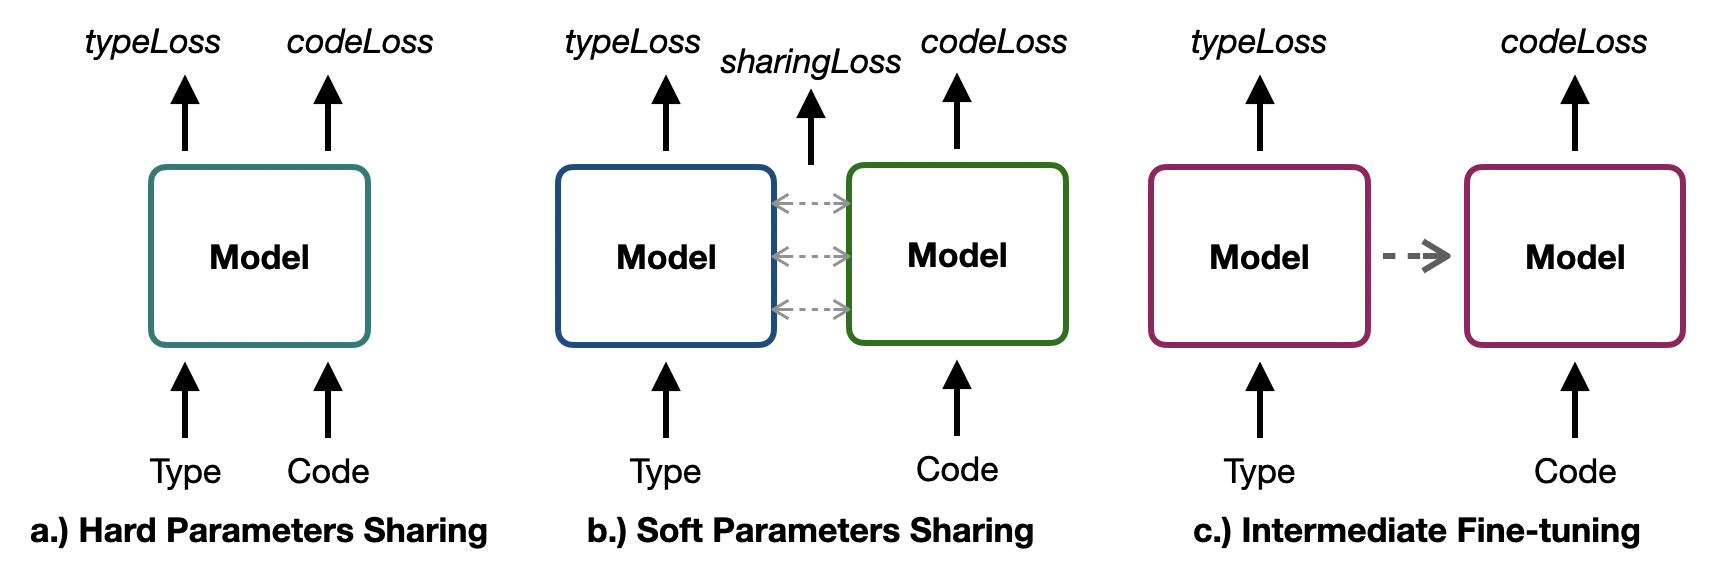
\includegraphics[width=\columnwidth]{figures/model_arch.png}
%     \caption{Model architectures (tentative pic)}
%     \label{fig:arch}
% \end{figure}   

   \subsection{(第五步)超参数任务加权}   
    \label{sec:approach-weight}   

由于我们的    \our    ~ 利用 MTL 训练技术同时学习多个不同的任务,因此某些任务可能比其他任务具有更高的影响力,稍后可能会为其他任务产生不令人满意的精度(称为冲突梯度问题)。为了防止任务之间出现这种梯度冲突,重要的是通过最小化损失来找到最佳任务权重。因此,我们优化超参数 (    $\alpha_i$    ) 来调整任务权重,从而为我们的架构找到最佳任务权重。具体来说,我们的目标是使用以下损失函数最小化代码预测任务以及类型预测任务的损失。

   \begin{equation}
    \label{eq:rq3}
    L_{MTL} = \argmin_{\omega}(\sum_{i}\alpha_i \cdot L_{i}(d, \omega))
\end{equation}   

   \subsection{(第六步)解码方法}   
    \label{sec:approach-decoding}   

解码是一种在生成序列时从潜在词汇表中选择下一个标记的方法。尽管仅选择最高可能的标记适合单个步骤,但它可能不是序列的最佳选择。由于下一个标记的搜索空间很大,不同的解码方法将有不同的机制,提供对下一个标记的不同预测。因此,解码方法的选择可能会影响我们的 ~    \our    的整体性能。在代码补全文献中,我们发现 Beam Search 是最常用的解码方法之一。然而,Holtzman~    \ea    ~    \cite{holtzman2019curious}    发现存在其他广泛用于 NLP 领域的解码方法,但在代码完成文献中仍大量探索。因此,我们的目标是试验以下六种解码方法。

   \begin{itemize}
    \item \textbf{Greedy} is a method to select the maximum probable vocabulary to be the next tokens.
    This method assumes that the model already outputs the best probability in every timestep.
    % it generates all possible tokens in the vocabulary list; then, it will choose top B candidates that have the most probability. Those B candidates will move to the next time step, and the process repeats. In the end, there will only be B candidates. The search space is only (10,000)*B.
%     Although selecting only the highest
% probability token is suitable for a specific time step, it
% might be a sub-optimal for a sequence. 
    
    \item \textbf{Beam Search} applies a search algorithm to generate all possible tokens in the vocabulary; then, it selects the top $b$ (i.e., beam size) probable tokens to continue.
    The Beam Search method is one of the most commonly used decoding methods in text generation tasks~\cite{li-etal-2016-deep, wiseman-etal-2017-challenges}.
    % However, Beam Search may not always achieve optimal results, since it does not consider the whole vocabulary, but instead only the top $b$ (i.e., beam size) probable tokens.
    % Nevertheless, Beam Search still performs faster than an exhaustive search.
    
    % ; however, it balances between the performance and the computational time.
    % The method's time complexity is equals to $O(b*V)$ where $V$ is the vocabulary size.
    % It . 
    
    % recommend the most probable $b$ next tokens according to a defined $b$ beam size threshold.

    
    
    
    % by expanding the graph in a limited set called beam~size~($b$).
    % In each timestep, the method generates all possible tokens in the vocabulary; then, it select the top $B$ probability tokens to continue.
      
    
    \item \textbf{Sampling} is a method to randomly select the next token from the actual probability distribution assigned by the model.
    Different from Greedy and Beam search methods which in some cases may recommend only the same probable next tokens at different timesteps, the sampling method may recommend different next tokens at different timesteps (i.e., non-deterministic).
    % We put the sampling method in this study as the baseline for other decoding methods. All of the methods that required sampling are set the seed value to the same number.
    
    % Temperature is used to increase the probability of probable tokens while reducing the one that is not. Usually, the range is 0 < temp ≤ 1. Note that when temp=1, there is no effect.
    \item \textbf{Sampling with Temperature} applies a temperature parameter to shape the probability distribution~\cite{ackley1985learning}, which is different from the original sampling method where the randomness is arbitrary.
    The temperature is used to increase the probability of the most probable next tokens, while decreasing the probability of the others.
    We note that the probability of the least probable next tokens is only decreased, but they are not removed from the recommendation.
    The range of the temperature value is usually at $0 < temp \le 1$, where $temp = 1$ is a normal sampling.

    % Additional to normal sampling which could be arbitrary, sampling with temperature method 
    \item \textbf{Top-K Sampling} aims to truncate the probability distribution by choosing the top-$k$ probable next tokens from the vocabulary, then, re-scale the distribution and perform sampling based on the new distribution.
    This method ensures that the less probable next tokens will not be generated, while only the top-$k$ probable next tokens are only considered during the sampling process.
    
    \item \textbf{Top-P Sampling (Nucleus Sampling)} is similar to the Top-k sampling method where the Top-P sampling method also truncates the probability distribution, but with different criteria. 
    Top-P sampling prunes the distribution by the cumulative probability of the current step $\ge p$~\cite{holtzman2019curious}; then, re-scale and perform sampling.
    Formally, given the probability P, we can define the smallest summation of the probability as $V_p$ in
    \begin{equation}
        \label{eq:top-p}
        \sum_{x\in V_p} P(x|x_{1:i-1}) \ge p
    \end{equation}
    The benefit of this method is that it can dynamically adjust the number of $k$ depending on the certainty of the model.
    If the model is very certain on some tokens, the search space is small, and vice versa.
\end{itemize}   

   \subsection{(第 7 步)代码完成}   
    \our    ~在两个粒度级别执行预测,即在令牌级别和行级别。

令牌级代码完成是一个预测下一个令牌(右侧)的过程,给定先前的代码令牌作为上下文(左侧)。

行级代码完成类似于令牌级预测,但该模型旨在预测下一个令牌,直到完成整行代码(即,不仅仅是一个下一个令牌)。对于行级预测,我们利用与令牌级代码完成任务相同的模型来迭代生成下一个令牌,其中新生成的令牌用作下一步预测的上下文。迭代地重复此过程,直到模型生成    $\langle EOL \rangle$    令牌,或直到达到某个    $n$    阈值(   $n=100$   ,遵循 CodeXGlue~   \cite{lu2021codexglue}   )。




\end{document}

